% Options for packages loaded elsewhere
\PassOptionsToPackage{unicode}{hyperref}
\PassOptionsToPackage{hyphens}{url}
%
\documentclass[
  oneside]{book}
\usepackage{amsmath,amssymb}
\usepackage{lmodern}
\usepackage{ifxetex,ifluatex}
\ifnum 0\ifxetex 1\fi\ifluatex 1\fi=0 % if pdftex
  \usepackage[T1]{fontenc}
  \usepackage[utf8]{inputenc}
  \usepackage{textcomp} % provide euro and other symbols
\else % if luatex or xetex
  \usepackage{unicode-math}
  \defaultfontfeatures{Scale=MatchLowercase}
  \defaultfontfeatures[\rmfamily]{Ligatures=TeX,Scale=1}
\fi
% Use upquote if available, for straight quotes in verbatim environments
\IfFileExists{upquote.sty}{\usepackage{upquote}}{}
\IfFileExists{microtype.sty}{% use microtype if available
  \usepackage[]{microtype}
  \UseMicrotypeSet[protrusion]{basicmath} % disable protrusion for tt fonts
}{}
\makeatletter
\@ifundefined{KOMAClassName}{% if non-KOMA class
  \IfFileExists{parskip.sty}{%
    \usepackage{parskip}
  }{% else
    \setlength{\parindent}{0pt}
    \setlength{\parskip}{6pt plus 2pt minus 1pt}}
}{% if KOMA class
  \KOMAoptions{parskip=half}}
\makeatother
\usepackage{xcolor}
\IfFileExists{xurl.sty}{\usepackage{xurl}}{} % add URL line breaks if available
\IfFileExists{bookmark.sty}{\usepackage{bookmark}}{\usepackage{hyperref}}
\hypersetup{
  pdftitle={Master-Thesis},
  pdfauthor={Axel Roth},
  hidelinks,
  pdfcreator={LaTeX via pandoc}}
\urlstyle{same} % disable monospaced font for URLs
\usepackage{color}
\usepackage{fancyvrb}
\newcommand{\VerbBar}{|}
\newcommand{\VERB}{\Verb[commandchars=\\\{\}]}
\DefineVerbatimEnvironment{Highlighting}{Verbatim}{commandchars=\\\{\}}
% Add ',fontsize=\small' for more characters per line
\usepackage{framed}
\definecolor{shadecolor}{RGB}{248,248,248}
\newenvironment{Shaded}{\begin{snugshade}}{\end{snugshade}}
\newcommand{\AlertTok}[1]{\textcolor[rgb]{0.94,0.16,0.16}{#1}}
\newcommand{\AnnotationTok}[1]{\textcolor[rgb]{0.56,0.35,0.01}{\textbf{\textit{#1}}}}
\newcommand{\AttributeTok}[1]{\textcolor[rgb]{0.77,0.63,0.00}{#1}}
\newcommand{\BaseNTok}[1]{\textcolor[rgb]{0.00,0.00,0.81}{#1}}
\newcommand{\BuiltInTok}[1]{#1}
\newcommand{\CharTok}[1]{\textcolor[rgb]{0.31,0.60,0.02}{#1}}
\newcommand{\CommentTok}[1]{\textcolor[rgb]{0.56,0.35,0.01}{\textit{#1}}}
\newcommand{\CommentVarTok}[1]{\textcolor[rgb]{0.56,0.35,0.01}{\textbf{\textit{#1}}}}
\newcommand{\ConstantTok}[1]{\textcolor[rgb]{0.00,0.00,0.00}{#1}}
\newcommand{\ControlFlowTok}[1]{\textcolor[rgb]{0.13,0.29,0.53}{\textbf{#1}}}
\newcommand{\DataTypeTok}[1]{\textcolor[rgb]{0.13,0.29,0.53}{#1}}
\newcommand{\DecValTok}[1]{\textcolor[rgb]{0.00,0.00,0.81}{#1}}
\newcommand{\DocumentationTok}[1]{\textcolor[rgb]{0.56,0.35,0.01}{\textbf{\textit{#1}}}}
\newcommand{\ErrorTok}[1]{\textcolor[rgb]{0.64,0.00,0.00}{\textbf{#1}}}
\newcommand{\ExtensionTok}[1]{#1}
\newcommand{\FloatTok}[1]{\textcolor[rgb]{0.00,0.00,0.81}{#1}}
\newcommand{\FunctionTok}[1]{\textcolor[rgb]{0.00,0.00,0.00}{#1}}
\newcommand{\ImportTok}[1]{#1}
\newcommand{\InformationTok}[1]{\textcolor[rgb]{0.56,0.35,0.01}{\textbf{\textit{#1}}}}
\newcommand{\KeywordTok}[1]{\textcolor[rgb]{0.13,0.29,0.53}{\textbf{#1}}}
\newcommand{\NormalTok}[1]{#1}
\newcommand{\OperatorTok}[1]{\textcolor[rgb]{0.81,0.36,0.00}{\textbf{#1}}}
\newcommand{\OtherTok}[1]{\textcolor[rgb]{0.56,0.35,0.01}{#1}}
\newcommand{\PreprocessorTok}[1]{\textcolor[rgb]{0.56,0.35,0.01}{\textit{#1}}}
\newcommand{\RegionMarkerTok}[1]{#1}
\newcommand{\SpecialCharTok}[1]{\textcolor[rgb]{0.00,0.00,0.00}{#1}}
\newcommand{\SpecialStringTok}[1]{\textcolor[rgb]{0.31,0.60,0.02}{#1}}
\newcommand{\StringTok}[1]{\textcolor[rgb]{0.31,0.60,0.02}{#1}}
\newcommand{\VariableTok}[1]{\textcolor[rgb]{0.00,0.00,0.00}{#1}}
\newcommand{\VerbatimStringTok}[1]{\textcolor[rgb]{0.31,0.60,0.02}{#1}}
\newcommand{\WarningTok}[1]{\textcolor[rgb]{0.56,0.35,0.01}{\textbf{\textit{#1}}}}
\usepackage{longtable,booktabs,array}
\usepackage{calc} % for calculating minipage widths
% Correct order of tables after \paragraph or \subparagraph
\usepackage{etoolbox}
\makeatletter
\patchcmd\longtable{\par}{\if@noskipsec\mbox{}\fi\par}{}{}
\makeatother
% Allow footnotes in longtable head/foot
\IfFileExists{footnotehyper.sty}{\usepackage{footnotehyper}}{\usepackage{footnote}}
\makesavenoteenv{longtable}
\usepackage{graphicx}
\makeatletter
\def\maxwidth{\ifdim\Gin@nat@width>\linewidth\linewidth\else\Gin@nat@width\fi}
\def\maxheight{\ifdim\Gin@nat@height>\textheight\textheight\else\Gin@nat@height\fi}
\makeatother
% Scale images if necessary, so that they will not overflow the page
% margins by default, and it is still possible to overwrite the defaults
% using explicit options in \includegraphics[width, height, ...]{}
\setkeys{Gin}{width=\maxwidth,height=\maxheight,keepaspectratio}
% Set default figure placement to htbp
\makeatletter
\def\fps@figure{htbp}
\makeatother
\setlength{\emergencystretch}{3em} % prevent overfull lines
\providecommand{\tightlist}{%
  \setlength{\itemsep}{0pt}\setlength{\parskip}{0pt}}
\setcounter{secnumdepth}{5}
\usepackage{booktabs}
\usepackage{amsthm}
\usepackage{amsmath}
\makeatletter
\def\thm@space@setup{%
  \thm@preskip=8pt plus 2pt minus 4pt
  \thm@postskip=\thm@preskip
}
\makeatother
\ifluatex
  \usepackage{selnolig}  % disable illegal ligatures
\fi
\usepackage[]{natbib}
\bibliographystyle{apalike}

\title{Master-Thesis}
\author{Axel Roth}
\date{2022-08-14}

\begin{document}
\maketitle

{
\setcounter{tocdepth}{1}
\tableofcontents
}
\hypertarget{preface}{%
\chapter*{Preface}\label{preface}}
\addcontentsline{toc}{chapter}{Preface}

\renewcommand{\chaptermark}[1]{\markboth{\uppercase{#1}}{\uppercase{#1}}}
\markboth{\uppercase{Preface}}{\uppercase{Preface}}

Blah blah blah

\renewcommand{\chaptermark}[1]{\markboth{\uppercase{\thechapter. \ #1}}{}}

\hypertarget{abstract}{%
\chapter{Abstract}\label{abstract}}

Things about this thesis. why and what question should be answered. and what are the answers. (zusammenfassung)

\hypertarget{software-information-and-usage}{%
\chapter{Software information and usage}\label{software-information-and-usage}}

wie ich das buch schreibe, R markodwn bookdown und so und welche versionen ich nutze

\hypertarget{r-version-and-packages}{%
\section{R-Version and Packages}\label{r-version-and-packages}}

\hypertarget{reproducibility}{%
\section{reproducibility}\label{reproducibility}}

github und code im bookdown

\hypertarget{r-functions}{%
\section{R-functions}\label{r-functions}}

zb plotly\_save

\hypertarget{open-data-sources}{%
\chapter{Open Data Sources}\label{open-data-sources}}

yahoo finance

\hypertarget{r-functions-1}{%
\section{R-functions}\label{r-functions-1}}

\hypertarget{mathematical-fundations}{%
\chapter{Mathematical Fundations}\label{mathematical-fundations}}

This chapter is a summary of mathematical calculations and conventions used in this Thesis. Its impotent to note that most mathematical formulas are expressed in matrix notation. Most of the time this will result in a direct translation into R-code. Additionally we state all assumptions needed for the modeled return structure, that can be easily used. It is important to say that the reality is too complex and can only partially be modeled. That is why we use fundamental and simple models that do not hold in practice. Nonetheless these models or improvements of it are widely used in finance and have proven to be useful. Additionally do these basic models produce more complex problems to solve by the PSO because for example factor models are often reduce the dimension of the dependency that are modeled.

\hypertarget{basic-operators}{%
\section{Basic Operators}\label{basic-operators}}

The following table is a compendium which will compare the used mathematical symbols to R-code and its meanings:

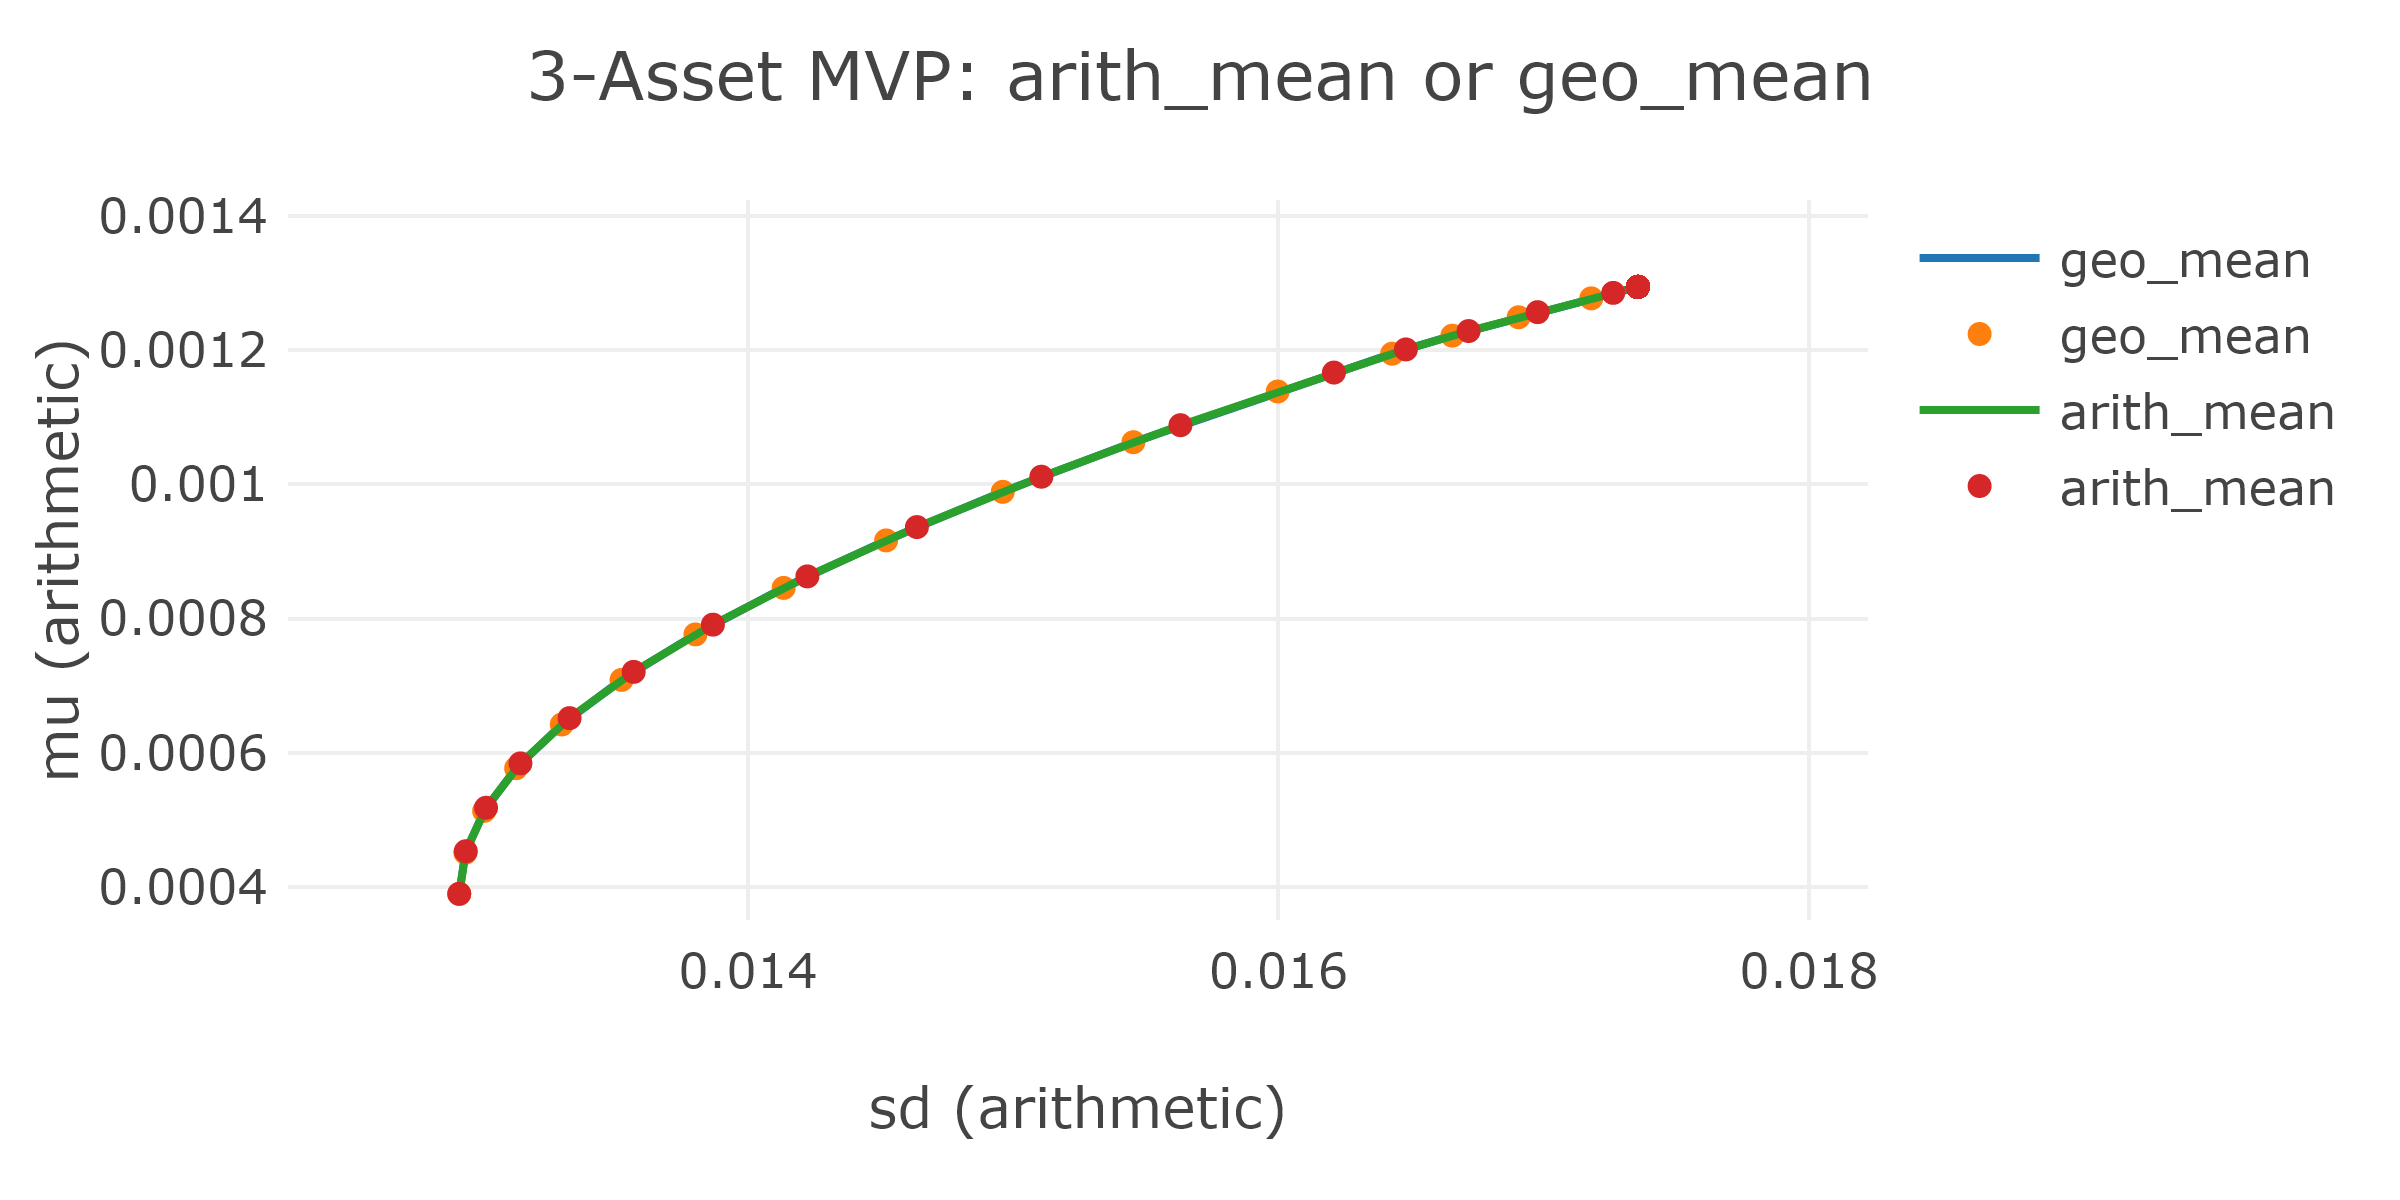
\includegraphics{Master_Thesis_files/figure-latex/unnamed-chunk-4-1.png}

\hypertarget{return-calculation}{%
\section{Return calculation}\label{return-calculation}}

Returns are fundamental for any portfolio optimization approach based on historical information. These returns reflect the percentage change from one point in time to another and are calculated from \href{https://www.investopedia.com/terms/a/adjusted_closing_price.asp}{adjusted closing prices}. Adjusted closing prices are reflecting dividends and are cleaned of by stock splits and rights offerings. These Returns enable the comparison of assets and are fundamental to analyze dependencies.

\hypertarget{daily-returns}{%
\subsection{daily returns}\label{daily-returns}}

We use exclusively simple returns in this thesis and the default timeframe for all rawdata is one workday. Suppose we have the adjusted closing price \(P\) of one asset on workday \(t_i\) and \(t_{i+1}\) so the simple returns can be calculated as follows:
\[
  R_{i+1} = \frac{P_{t_{i+1}}}{P_{t_i}}-1
\]

\hypertarget{annualized-returns}{%
\subsection{annualized returns}\label{annualized-returns}}

\hypertarget{markowitz-modern-portfolio-theory-mpt}{%
\section{Markowitz Modern Portfolio Theory (MPT)}\label{markowitz-modern-portfolio-theory-mpt}}

Harry Markowitz published his first groundbreaking work at 1952 and had a huge impact on the current financial point of view. Mainly by describing the impact of diversification and efficient portfolios. Efficient portfolios are those who have minimum risk for the given expected return or maximum expected return for a given risk target. Diversification can be described as ``a portfolio has the same return but less variance as the sum of its parts''. This holds if the assets are not perfectly correlated because bad and good movers can compensate each other which will result in a reduction of extreme situations. More detailed information can be found at \citep{Mari2005}.

\hypertarget{assumptions-of-markowitz-portfolio-theory}{%
\subsection{Assumptions of Markowitz Portfolio Theory}\label{assumptions-of-markowitz-portfolio-theory}}

A good summarirization of Markowitz assumptions can be found in \citep{Mari2005}:

\begin{enumerate}
    \item perfect market without taxes or transaction costs.
    \item short sales are disallowed.
    \item assets are infinitely divisible.
    \item Expected Returns, Variances and Covariances contain all information.
    \item Investors are risk-adverse, they will only accept greater risk if they
are compensated with a higher expected return.
\end{enumerate}

It is not necessary to assume that the returns are normally distributed, but we will use it here, to simplify the problem. More information about the conditions for using other distributions can be found in \citep{Mari2005}. It is clear that these assumption do not hold in practice.

\hypertarget{portfolio-math}{%
\section{Portfolio Math}\label{portfolio-math}}

This Section will provide proofs for the basic calculations needed for portfolio optimization like shown in \citep{Eric2021}. Hopefully this will enable all readers to understand the stated formulas completely. We prefer a different notation of the returns than in most sources, because its the common data-format used in practice. The used notations are the random return vector \(R\) and the portfolio weights \(w\) for \(N\) assets:
\[
  R = 
  \begin{bmatrix}
    R_{1} & R_{2} & \cdots & R_{N}  
 \end{bmatrix}
 , \ \ 
 w = 
  \begin{bmatrix}
    w_{1} \\ 
    w_{2} \\
    \cdots \\
    w_{N}  
 \end{bmatrix}
\]
And we simplify each return to be normally distributed with \(R_i = \mathcal{N}(\mu_i, \sigma_i^2)\) in this thesis. QUELLLLEEEEE It follows that linear combinations of normally distributed random variables are jointly normal distributed and can be fully described by its mean, variance and covariance.

\hypertarget{expected-returns}{%
\subsection{expected returns}\label{expected-returns}}

The expected returns of the vector of normal distributed random variables \(R \in \mathbb{R}^{N}\) can be calculated as follows:
\[
  E[R] =
  \begin{bmatrix}
    E[R_{1}] & E[R_{2}] & \cdots & E[R_{N}]  
 \end{bmatrix}
 =
 \begin{bmatrix}
    E[\mu_{1}] & E[\mu_{2}] & \cdots & E[\mu_{N}]  
 \end{bmatrix}
 =
 \mu
\]
\#\#\# expected portfolio return
The linear combination of the expected returns \(\mu\) with a weighting vector \(w\) (e.g.~portfolio weights) can be calculated as follows:
\[
 \mu \times w =
  \begin{bmatrix}
    E[\mu_{1}] & E[\mu_{2}] & \cdots & E[\mu_{N}]
 \end{bmatrix}
  \times 
  \begin{bmatrix}
    w_{1} \\ 
    w_{2} \\
    \cdots \\
    w_{N}  
 \end{bmatrix}
 =
 E[\mu_{1}] \cdot w_1 + E[\mu_{2}] \cdot w_2 + \cdots + E[\mu_{N}] \cdot w_{N} 
 =
 \mu_P
\]

\hypertarget{portfolio-returns}{%
\subsection{portfolio returns}\label{portfolio-returns}}

Let \(R \in \mathbb{R}^{T \times N}\) denote a realized return Matrix of \(N\) assets and \(T\) days in the past. The portfolio return on each day can be calculated with the formula of the expected portfolio return. On all days \(T\) can this be done by:
\[
  R \times w = 
  \begin{bmatrix}
    R_{1, 1} & R_{1, 2} & \cdots & R_{1, N} \\
    R_{2, 1} & R_{2, 2} & \cdots & R_{2, N} \\
    \cdots \\
    R_{T, 1} & R_{T, 2} & \cdots & R_{T, N} \\
 \end{bmatrix}
  \times 
  \begin{bmatrix}
    w_{1} \\ 
    w_{2} \\
    \cdots \\
    w_{N}  
 \end{bmatrix}
 =
   \begin{bmatrix}
    R_{1}^P \\ 
    R_{2}^P \\
    \cdots \\
    R_{N}^P  
 \end{bmatrix}
 =
 R_P
\]

\hypertarget{activ-vs-passiv-investing}{%
\chapter{Activ vs Passiv Investing}\label{activ-vs-passiv-investing}}

The fundation of each Asset Management

passiv vs activ studie
\texttt{https://www.scirp.org/journal/paperinformation.aspx?paperid=92983}

gut gut
\url{file:///C:/Users/Axel/Desktop/Master-Thesis-All/Ziel\%20was\%20beantwortet\%20werden\%20soll/Quellen\%20nur\%20wichtige/Rasmussen2003_Book_QuantitativePortfolioOptimisat.pdf}

\begin{Shaded}
\begin{Highlighting}[]
\FunctionTok{source}\NormalTok{(}\StringTok{"global.R"}\NormalTok{)}
\NormalTok{knitr}\SpecialCharTok{::}\NormalTok{opts\_chunk}\SpecialCharTok{$}\FunctionTok{set}\NormalTok{(}\AttributeTok{cache =}\NormalTok{ T, }\AttributeTok{warning=}\NormalTok{F, }\AttributeTok{message=}\NormalTok{F)}
\end{Highlighting}
\end{Shaded}

\hypertarget{challenges-of-passiv-investing}{%
\chapter{Challenges of Passiv Investing}\label{challenges-of-passiv-investing}}

In this Chapter we will discuss two common challenges of Passiv-Investing and create simple examples to test the PSO. The first one is the mean-variance portfolio (MVP) from the modern portfolio theory of Markowitz which is simply said an optimal allocation of assets regarding risk and return. The second challenge is the index-tracking-problem which tries to construct a portfolio which has a minimal tracking error to a given benchmark.

\hypertarget{mean-variance-portfolio-mvp}{%
\section{Mean-variance portfolio (MVP)}\label{mean-variance-portfolio-mvp}}

Markowitz has shown that diversifying the risk on multiple assets will reduce the overall risk of the portfolio. This result was the beginning of the widely used modern portfolio theorie which uses mathematical models to archive portfolios with minimal variance for a given return target. All these optimal portfolios for a given return target are called efficient and create the efficient frontier.

\hypertarget{mvp}{%
\subsection{MVP}\label{mvp}}

We have \(N\) assets and its returns on \(T\) different days which creates a return matrix \(R \in \mathbb{R}^{T \times N}\). Each element \(R_{t,i}\) contains the return of the \(i\)-th asset on day \(t\). The covariance matrix of the returns is \(\textstyle\sum \in \mathbb{R}^{N \times N}\) and the expected returns are \(\mu \in \mathbb{R}^{N}\). The MVP with risk aversion parameter \(\lambda \in [0,1]\) like shown in \citep{Mari2005} can be formalized as follows:
\begin{equation} 
\underset{w}{minimize} \ \ \ \lambda \ w^T \textstyle\sum w - (1-\lambda) \ \mu^T w
\label{eq:MVP}
\end{equation}

The risk aversion parameter \(\lambda\) defines the trade-off between risk and return. With \(\lambda = 1\), the minimization problem only contains the the variance term and so on results in a minimum variance portfolio and \(\lambda = 0\) transforms the problem to a minimization of the negative expected returns so on results in a maximum return portfolio. All possible \(\lambda \in [0, 1]\) represent the efficient frontier.

\hypertarget{mvp-example}{%
\subsection{MVP example}\label{mvp-example}}

We will analyze a small example to understand the meaning of the efficient frontier without going into detail how it was solved. First of all we are loading the daily returns of IBM, Google and Apple from the year 2020.

The cumulated daily returns are:

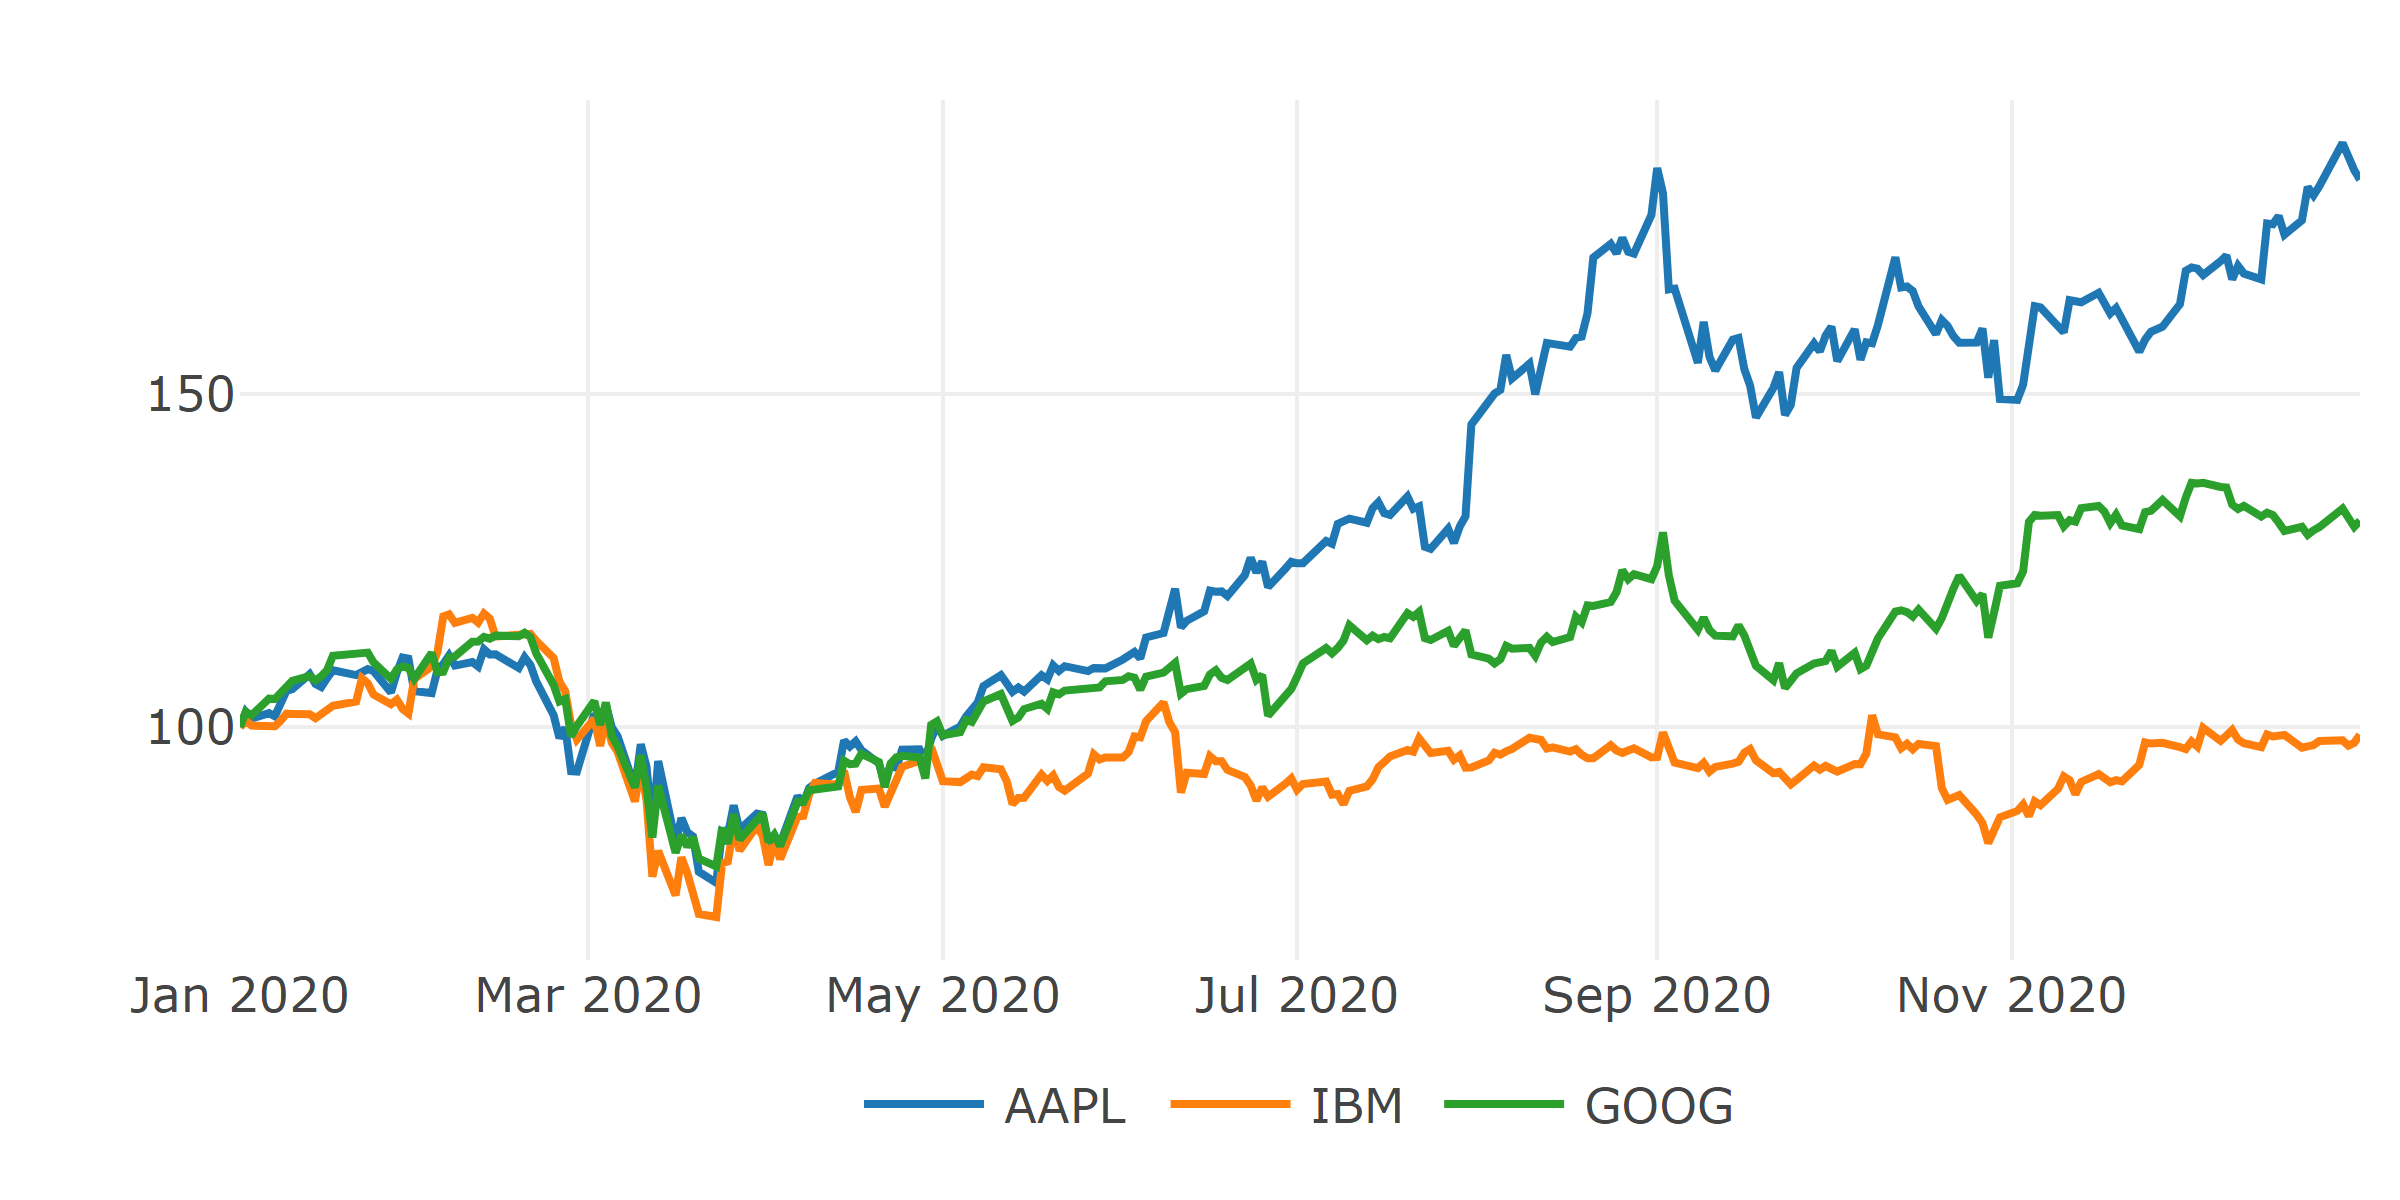
\includegraphics{Master_Thesis_files/figure-latex/unnamed-chunk-7-1.png}

Now we can calculate the expected daily returns and the covariance matrix for the 3 assets:

\begin{Shaded}
\begin{Highlighting}[]
\NormalTok{mu }\OtherTok{\textless{}{-}} \FunctionTok{as.vector}\NormalTok{((}\FunctionTok{last}\NormalTok{(}\FunctionTok{ret\_to\_cumret}\NormalTok{(returns))}\SpecialCharTok{/}\DecValTok{100}\NormalTok{)}\SpecialCharTok{\^{}}\NormalTok{(}\DecValTok{1}\SpecialCharTok{/}\FunctionTok{nrow}\NormalTok{(returns))}\SpecialCharTok{{-}}\DecValTok{1}\NormalTok{) }\SpecialCharTok{\%\textgreater{}\%} 
  \FunctionTok{setNames}\NormalTok{(., }\FunctionTok{colnames}\NormalTok{(returns))}
\NormalTok{mu}
\end{Highlighting}
\end{Shaded}

\begin{verbatim}
##           AAPL            IBM           GOOG 
##  0.00237641721 -0.00004622149  0.00106873786
\end{verbatim}

\begin{Shaded}
\begin{Highlighting}[]
\NormalTok{cov }\OtherTok{\textless{}{-}} \FunctionTok{as.matrix}\NormalTok{(}\FunctionTok{nearPD}\NormalTok{(}\FunctionTok{cov}\NormalTok{(returns))}\SpecialCharTok{$}\NormalTok{mat)}
\NormalTok{cov}
\end{Highlighting}
\end{Shaded}

\begin{verbatim}
##              AAPL          IBM         GOOG
## AAPL 0.0008635696 0.0004356282 0.0005337719
## IBM  0.0004356282 0.0006626219 0.0004086728
## GOOG 0.0005337719 0.0004086728 0.0005827306
\end{verbatim}

We now have all the necessary data to solve the MVP \eqref{eq:MVP} with \(\lambda \in \{0.01, 0.02, ..., 0.99, 1\}\). We calculate all 100 portfolios by solving the quadratic minimization problem for each \(\lambda\).

Following that, we convert the daily returns and standard deviation to yearly returns and standard deviation before plotting the efficient frontier.

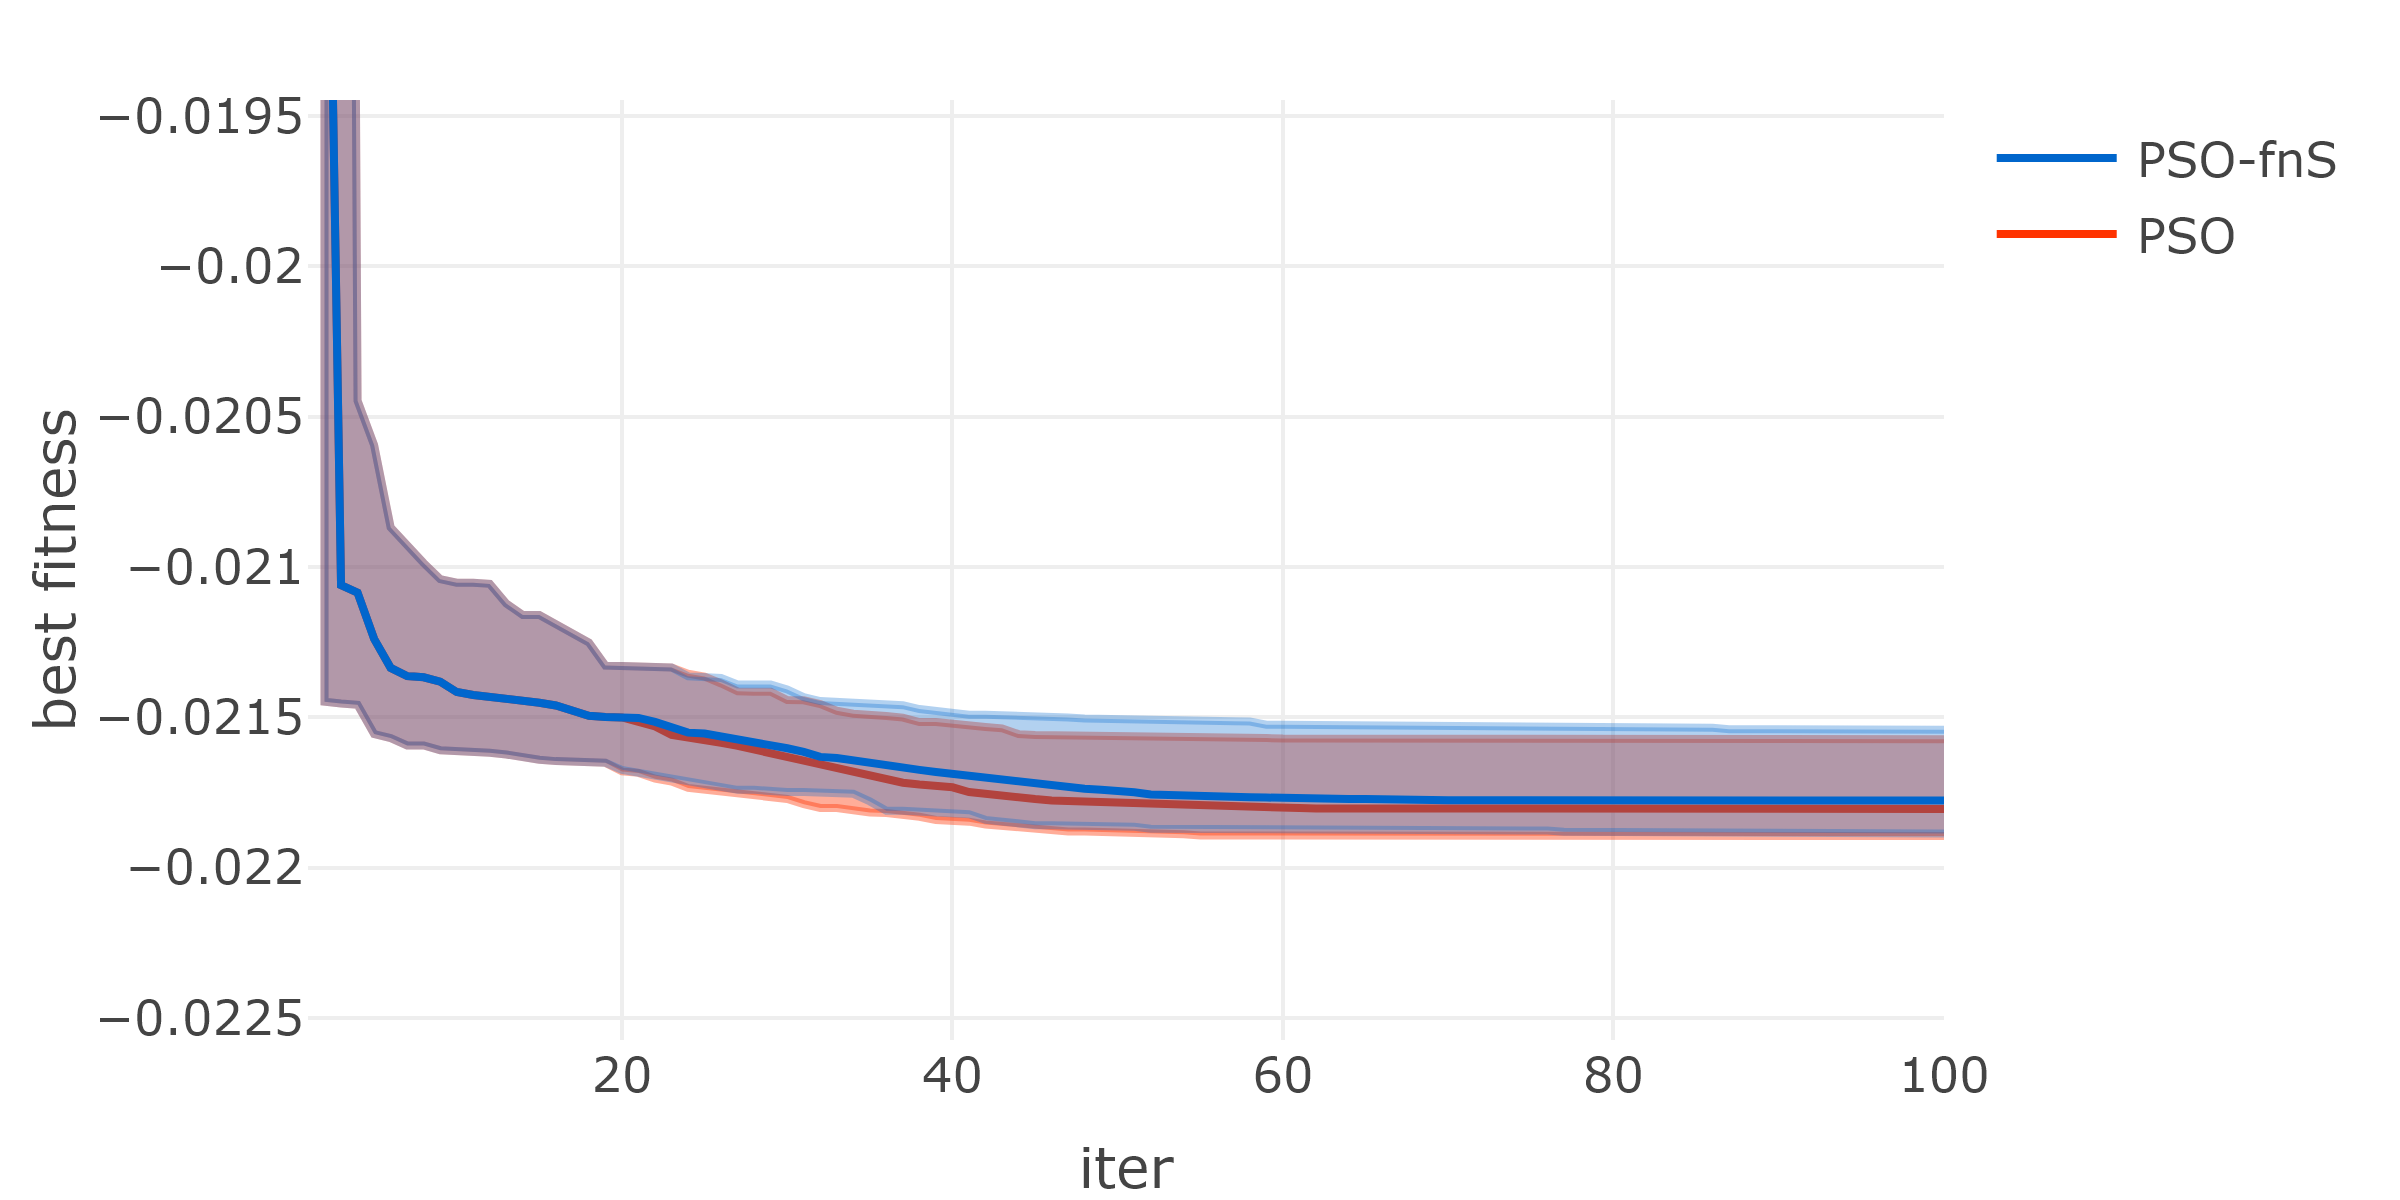
\includegraphics{Master_Thesis_files/figure-latex/unnamed-chunk-10-1.png}

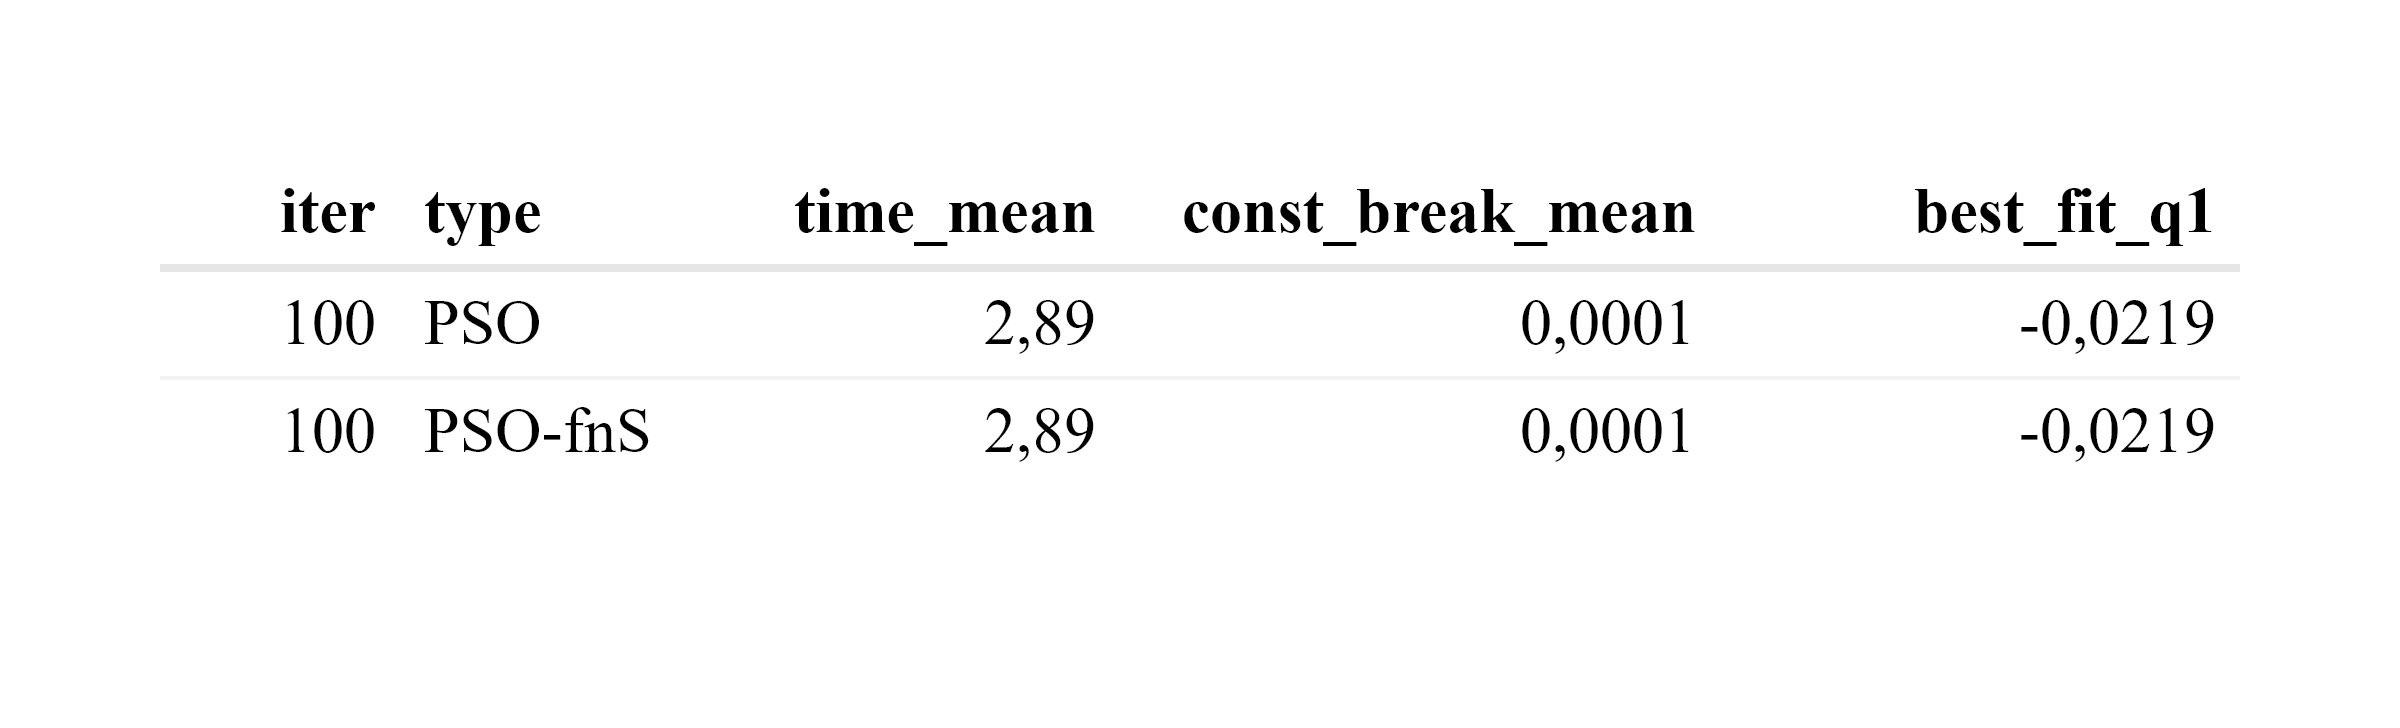
\includegraphics{Master_Thesis_files/figure-latex/unnamed-chunk-11-1.png}

\hypertarget{index-tracking-portfolio-itp}{%
\section{Index-tracking portfolio (ITP)}\label{index-tracking-portfolio-itp}}

Indices are asset baskets that are used to track the performance of a specific asset group. The well-known Standard and Poor's 500 index (short: S\&P 500), for example, tracks the top 500 stocks in the United States. All indices are not investible and only serve to visualize the performance of these asset groups without incurring transaction costs. Asset managers use such indices as benchmarks to compare the performance of their funds. Each fund has its own benchmark, which contains roughly the same assets that the manager could purchase. If the fund underperforms its benchmark, it may be an indication that the fund manager made a poor decision. That is why all fund managers strive to outperform their benchmarks through carefully chosen investments. The past has proven that this is rearly achived with activ managemnt after costs \citep{Desm2016}. This is the reason why passiv managed funds with the goal to track there benchmarks are becoming more frequent. This is why passively managed funds with the purpose of tracking their benchmarks are becoming more common. This can be accomplished through either full or sparse replication. In most circumstances, a full replication that achieves the exact performance we seek is not achievable because not all assets in an index are investable. And, if so, it would be unwise because benchmarks with numerous indexes can contain over ten thousand separate assets, resulting in a massive amount of transaction costs. A sparse replication of the performance is the most prevalent approach. To do so, the portfolio manager must define his benchmark, which should overlap with his fund's investing universe. Following that, he will reduce this universe using investor principles such as liquidity and availability. Now he can begin to optimize a portfolio, taking into account the investor constraints, in order to match the benchmark performance. Typically, this is accomplished by lowering the variance between the ITP's daily returns and the benchmark:

\[
 minimize \ \ Var(r_{p}-r_{bm})
\]

To obtain the portfolio weights \(w\), we must first substitute \(r_{p}\) as shown below:

\[
  r_{p} = R * w
\]

The Variance is then solved up until a quadratic problem dependent on the portfolio weights \(w\) is represented:

\[
 Var(r_{p}-r_{bm}) = Var(R * w - r_{bm}) = Var(R * w) + Var(r_{bm}) - 2 \cdot Cov(R*w,r_{bm}) 
\]
We must now solve each of the three terms, beginning with the easiest.

\[
Var(r_{bm}) = \sigma_{bm}^2 = constant
\]

The variance of the portfolio can be solved by looking at the Portfolio math Using Matrix Algebra section in \citep{Eric2021}:

\[
Var(R * w) = w^T * Cov(R) * w
\]

And the last term can be solved in general as (\url{https://bookdown.org/compfinezbook/introcompfinr/Multivariate-Probability-Distributions-Using-Matrix-Algebra.html} 3.6.5):

\[
  Cov(A*a, b) = Cov(b, A*a) = E[(b-\mu_{b})(A*a-\mu_{A}*a)] = E[(b-\mu_{b})(A-\mu_{A})*a] = E[(b-\mu_{b})(A-\mu_{A})]*a = Cov(A,b) * a
\]

\begin{Shaded}
\begin{Highlighting}[]
\NormalTok{A }\OtherTok{=} \FunctionTok{matrix}\NormalTok{(}\FunctionTok{c}\NormalTok{(}\DecValTok{1}\NormalTok{,}\DecValTok{4}\NormalTok{,}\DecValTok{2}\NormalTok{,}\DecValTok{4}\NormalTok{,}\DecValTok{6}\NormalTok{,}\DecValTok{3}\NormalTok{,}\DecValTok{8}\NormalTok{,}\DecValTok{4}\NormalTok{,}\DecValTok{4}\NormalTok{,}\DecValTok{10}\NormalTok{), }\AttributeTok{ncol=}\DecValTok{2}\NormalTok{)}
\NormalTok{a }\OtherTok{=} \FunctionTok{c}\NormalTok{(}\FloatTok{0.2}\NormalTok{, }\FloatTok{0.8}\NormalTok{)}
\NormalTok{b }\OtherTok{=} \FunctionTok{c}\NormalTok{(}\DecValTok{4}\NormalTok{,}\DecValTok{4}\NormalTok{,}\DecValTok{5}\NormalTok{,}\DecValTok{5}\NormalTok{,}\DecValTok{7}\NormalTok{)}

\FunctionTok{cov}\NormalTok{(A }\SpecialCharTok{\%*\%}\NormalTok{ a, b)}
\end{Highlighting}
\end{Shaded}

\begin{verbatim}
##      [,1]
## [1,] 2.15
\end{verbatim}

\begin{Shaded}
\begin{Highlighting}[]
\FunctionTok{t}\NormalTok{(a) }\SpecialCharTok{\%*\%} \FunctionTok{cov}\NormalTok{(A, b)}
\end{Highlighting}
\end{Shaded}

\begin{verbatim}
##      [,1]
## [1,] 2.15
\end{verbatim}

\begin{Shaded}
\begin{Highlighting}[]
\FunctionTok{t}\NormalTok{(}\FunctionTok{cov}\NormalTok{(A, b)) }\SpecialCharTok{\%*\%}\NormalTok{ a }\CommentTok{\# das hier wird gebraucht}
\end{Highlighting}
\end{Shaded}

\begin{verbatim}
##      [,1]
## [1,] 2.15
\end{verbatim}

This results in the final formula of the ITP:

\begin{equation}
  \begin{split}
   Var(r_{p}-r_{bm}) & = Var(R \times w - r_{bm}) \\
   & = Var(R \times w) - 2 \cdot Cov(R \times w,r_{bm}) + Var(r_{bm})  \\
   & = w^T \times Cov(R) \times w - 2 \cdot Cov(r_{bm}, R)^T \times w + \sigma_{bm}^2
   \end{split}
   \label{eq:ITP}
\end{equation}

The minimization problem of the ITP in the general stricture which all optimizers need is:

\[
  min(\frac{1}{2} \cdot b^T \times D \times b -d^T \times b)
\]

Because it is a minimization we can ignore constant terms and stretching coefficients and still find the same minimum. This results in the general substitution of the ITP as follows:

\[
  D = Cov(R)
\]

and

\[
d = Cov(r_{bm}, R)
\]

Now we need to add some basic constraints like in the MVP, to sum up the weights to 1 and being long only.

\hypertarget{example-itp}{%
\subsection{Example ITP}\label{example-itp}}

We will show the results of tracking the S\&P 500 with a tracking portfolio that can only invest in IBM, Apple and Google without going into details:

\begin{verbatim}
##      AAPL       IBM      GOOG 
## 0.2677928 0.4041880 0.3280192
\end{verbatim}

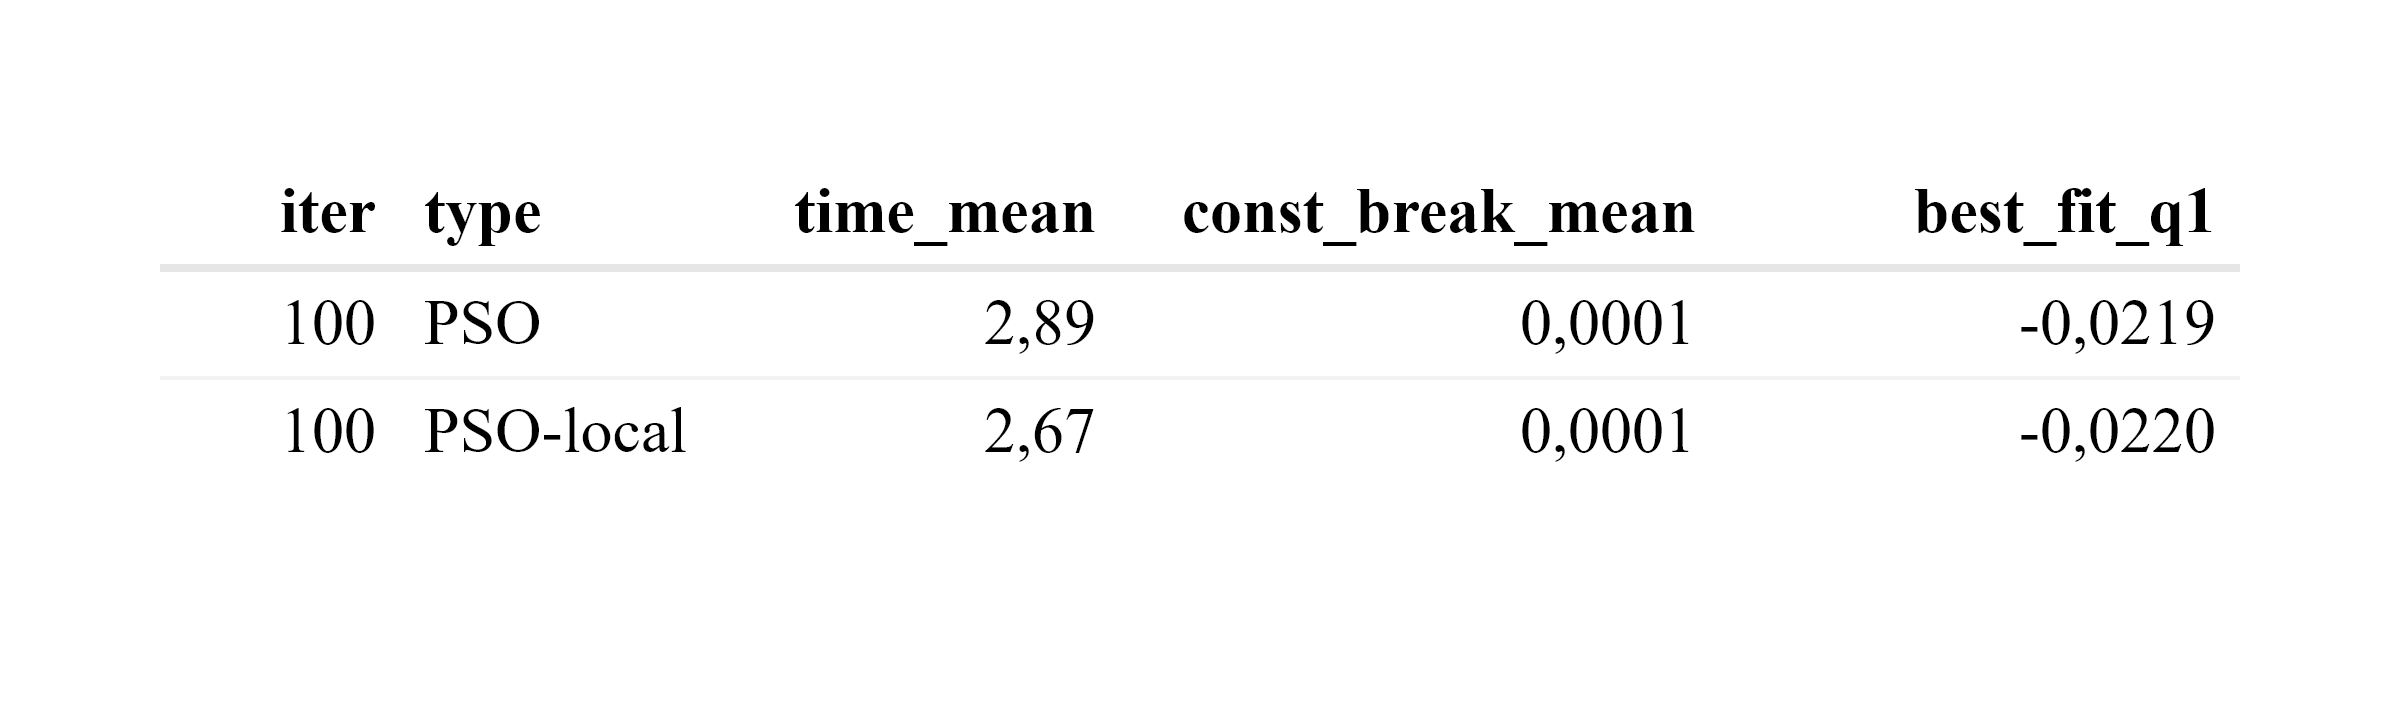
\includegraphics{Master_Thesis_files/figure-latex/unnamed-chunk-13-1.png}

\hypertarget{analytical_solver}{%
\chapter{Analytical\_Solver}\label{analytical_solver}}

example to solve problems with analytical solvers

\hypertarget{simple_particle_swarm_optimization}{%
\chapter{Simple\_Particle\_Swarm\_Optimization}\label{simple_particle_swarm_optimization}}

first pso examples and explainations

  \bibliography{book.bib,packages.bib}

\end{document}
